\section{The ATLAS Experiment}
ATLAS (A Toroidal LHC ApparatuS) is one of two general purpose detectors at CERN (the European Organization for Nuclear Research) near Geneva in Switzerland. These detectors collect data from the collisions provided by the worlds highest energy particle accelerator~\cite{lhc-design-report}, the Large Hadron Collider (LHC) situated at CERN. \\

In this section, information about the LHC and the ATLAS detector are given. This includes technical aspects of the ATLAS detector and the processing of data into meaningful physics objects to be used in analyses. The following chapter consists of information from "The LHC Design Report"~\cite{lhc-design-report}, "LHC Machine"~\cite{Evans_2008} and "The ATLAS Experiment at the CERN Large Hadron Collider"~\cite{Collaboration_2008} unless otherwise stated.

\subsection{Large Hadron Collider (LHC)}
The LHC is a circular 27 km particle accelerator located in an underground tunnel on the border between France and Switzerland. The accelerator consists of supercooled, superconducting magnets which accelerate and collide beams of protons at centre-of-mass energies up to $\sqrt{s} = 13$ TeV at instantaneous luminosities of $\mathcal{L} \sim 10^{34}$ cm$^{-2}$s$^{-1}$. In the LHC, $pp$ beams consist of bunches of protons which collide every 25 ns, corresponding to a frequency of 40 MHz. Several accelerator systems are used to accelerate protons and heavy ions to such high energies. Protons are extracted from a tank of ionised hydrogen gas and are injected into the Linear Accelerator 2 (LINAC), where they are linearly accelerated to momenta of 50 MeV. The proton bunches are then sequentially accelerated by a chain of circular accelerators. The chain starts with the Booster which accelerates the protons to momenta of up to 1.4 GeV. The proton bunches are then fed through to the Proton Synchrotron (PS) and the Super Proton Synchrotron (SPS) which accelerate the protons to momenta of up to 25 GeV and 450 GeV respectively. The protons are then transferred to two beam pipes of the LHC where they travel in opposite directions. Both proton beams are accelerated to their final momenta of 6.5 TeV, resulting in a centre-of-mass energy of 13 TeV. These proton beams then collide at one of the four main interaction points (positions along the beam pipe where collisions occur) situated along the LHC. \\

The four main experiments located at the interaction points are ATLAS, the Compact Muon Solenoid (CMS), Large Hadron Collider Beauty (LHCb) Experiment and A Large Ion Collider Experiment (ALICE). ATLAS and CMS are general-purpose detectors which investigate a wide range of physics processes. Since both ATLAS and CMS can measure the same processes, they are able to cross-check and validate measurements taken by one another. LHCb is specifically designed to study decays of particles containing $b$-quarks. ALICE is designed to study the strongly interacting quark-gluon plasma which is formed at extremely high energy densities. At the interaction points, the two proton beams which consist of protons in closely packed bunches, travel in opposite directions to one another and collide. We are only able to study one $pp$ collision (event) at a time, however many hard $pp$ collisions can occur per bunch crossing. These additional collisions are referred to as \textit{pile-up}. Pileup complicates the reconstruction of the particles originating from the hard collision of interest. 

\subsubsection{Luminosity}
This section consists of information from "Modern Particle Physics"~\cite{thomson2013modern}, unless otherwise stated.\\

The event production rate at the LHC, $R(t)$, for a certain process of interest is given by, 

\begin{equation}
R(t) = \mathcal{L}(t)\sigma
\end{equation}
where $\mathcal{L}(t)$ is the instantaneous luminosity and $\sigma$ and is the cross section of the process of interest. The instantaneous luminosity, $\mathcal{L}(t)$, is independent on the process of interest, and depends on various collider and beam parameters. $\mathcal{L}(t)$ can be written in terms of these parameters as,

\begin{equation}
\mathcal{L}(t) = f \frac{N n_{1} n_{2}}{4\pi \sigma_{x} \sigma_{y}}
\end{equation}

where $f$ is the beam revolution frequency, $N$ is the number of proton bunches colliding per second, $n_{1}$ and $n_{2}$ are the number of protons in the colliding bunches, $\sigma_{x}$ and $\sigma_{y}$ are the beam spread in the $x$ and $y$ directions respectively. The total integrated luminosity, $L$, across some time interval, is given by,

\begin{equation}
L = \int \mathcal{L} dt.
\end{equation}
The units of $L$ are inverse area, and are given by fb$^{-1}$ at the LHC and the ATLAS detector. In Figure~\ref{fig:lhc-lumi}, the total integrated luminosity delivered to ATLAS, recorded by ATLAS, and certified to be good enough for physics analyses (the data passes certain quality control criteria) for $\sqrt{s} = 13$ TeV $pp$ collisions at the LHC is shown~\cite{LHC-lumi}. 

\begin{figure}[h!]
 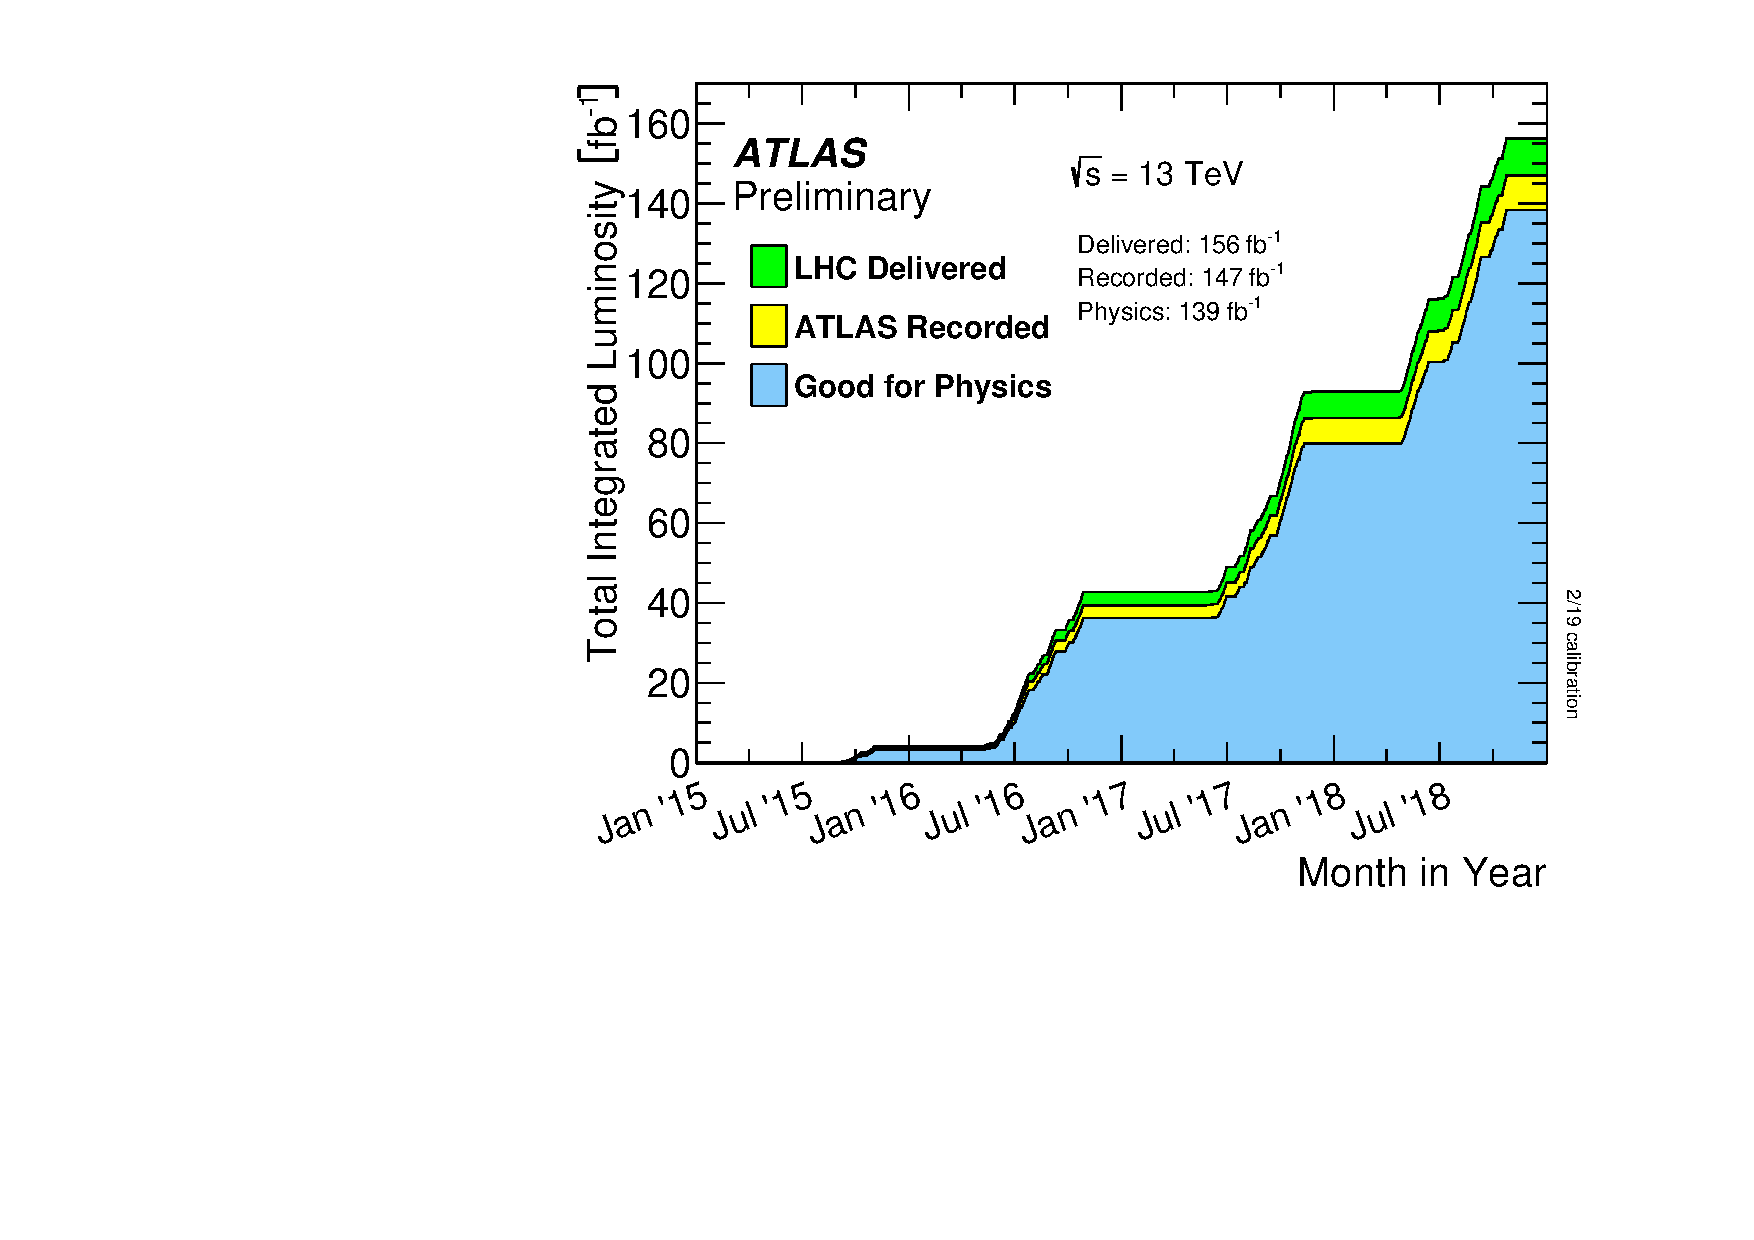
\includegraphics[width=0.5\textwidth]{figures/theoryFigs/lhc_lumi.pdf}
 \centering
\caption{The total integrated luminosity delivered to ATLAS, recorded by ATLAS, and certified to be good enough for physics analyses (the data passes certain quality control criteria) for $\sqrt{s} = 13$ TeV $pp$ collisions at the LHC is shown~\cite{LHC-lumi}. The total integrated luminosity delivered by the LHC, recorded by ATLAS and certified to be good quality data are shown by the green, yellow and blue histograms respectively. The month and year of data taking is shown on the x-axis and the total integrated luminosity (in fb$^{-1}$) is shown on the y-axis.}
\label{fig:lhc-lumi}
\end{figure}

A total integrated luminosity of 139 fb$^{-1}$ of data certified as good for physics was recorded by ATLAS between 2015 and 2018. This data taking period is referred to as Run 2, since it proceeds the Run 1 data taking period (2011 and 2012) and the Long Shutdown 1 LHC upgrade period (2013 and 2014). In this analysis, we use the Full Run 2 dataset.


\section{The ATLAS Detector}
In Figure~\ref{fig:atlas-detector}, the schematic of the ATLAS detector, is shown.

\begin{figure}[h!]
 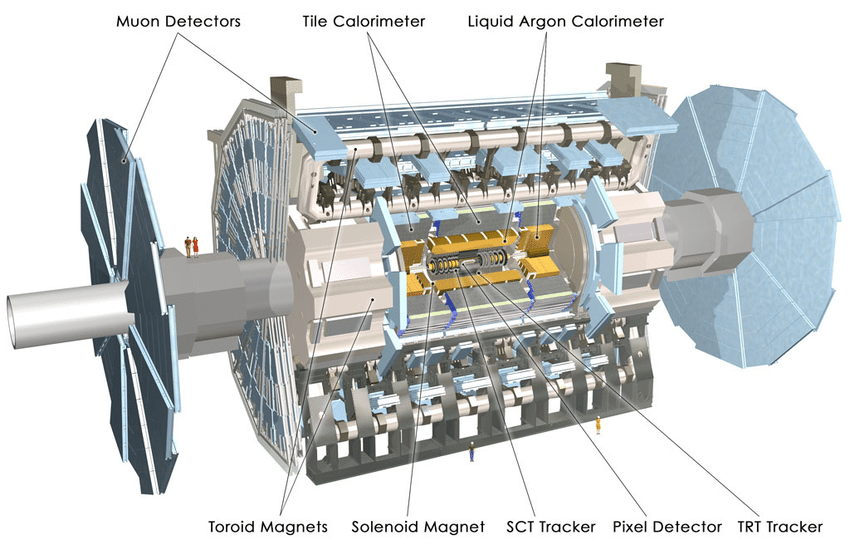
\includegraphics[width=0.5\textwidth]{figures/theoryFigs/atlasDetector.png}
 \centering
\caption{Schematic of the ATLAS detector~\cite{Collaboration_2008}}
\label{fig:atlas-detector}
\end{figure}

The detector is cylindrically shaped which covers close to 4$\pi$ in solid angle. It has a length of 44 m, a diameter of 25 m and a mass of 7000 tons. ATLAS consists of four main sub-detectors arranged in concentric cylindrical layers around the beam pipe. These include the inner detector, the electromagnetic calorimeter, the hadronic calorimeters and the muon spectrometer. The sub-detectors record the momenta, energies and trajectories of different particles produced in the collider, allowing for the reconstruction and identification of these particles to be used in physics analyses.

\subsection{Coordinate System and Kinematics}

The ATLAS detector adopts a right-handed coordinate system. The origin is at the nominal interaction point with the beam direction defining the $z-$axis. The $x-y$ plane (or transverse plane) is perpendicular to the beam line, with the $x-$axis pointing towards the centre of the LHC ring and the $y$-axis pointing upwards towards the Earth's surface. The azimuthal angle, $\phi \in [-\pi, \pi]$, is measured in the transverse plane with respect to the positive $x-$axis. The polar angle, $\theta \in [0,\pi]$, is measured in the $z-y$ plane with respect to the positive $y-$axis. A quantity called the pseudorapidity, $\eta \in [0,\infty]$ is defined as,

\begin{equation}
\eta = -\ln{\tan{\left(\frac{\theta}{2}\right)}}
\end{equation}
$\eta$ is often used as a measure of the polar angle, instead of $\theta$, since the difference in $\eta$ between two particles, $\Delta \eta$, is invariant under a Lorentz boost in the $z-$direction~\cite{Tovey_2019}. The angular distance between two physics objects, $\Delta R$, can be written as,

\begin{equation}
\Delta R = \sqrt{(\Delta\phi)^{2} + (\Delta\eta)^{2}}
\end{equation}
where $\Delta\phi$ is the difference in $\phi$ between the two physics objects of interest. Quantities defined in the transverse plane are often used to describe the kinematics of physics objects in hadron collider experiments. The transverse momentum, $p_{T}$, is defined as,
\begin{equation}
p_{T}= \sqrt{(p_{x})^{2} + (p_{y})^{2}}
\end{equation}
where $p_{x}$ and $p_{y}$ are the $x$ and $y$ components of the physics object's momenta, respectively. The transverse energy, $E_{T}$, is defined as,
\begin{equation}
E_{T} = \sqrt{m^{2} + p_{T}^{2}}
\end{equation}
where $m$ is the invariant mass of the physics object. 

%The energy and momentum in particle collisions are conserved, however the absence of detector elements along the beam line, neutrinos escaping from the detector and unknown initial parton momenta restricts us from fully reconstructing the initial and final state particles. We can however, quantify the amount of transverse momenta which is - possibly go in particle ID section


\subsection{Inner Detector}
The inner detector is the first layer of concentric cylindrical sub-detector layers in the ATLAS detector. It is used to identify charged particles and reconstruct the trajectories of charged particles produced in the collisions via energy deposition in semiconductor material (hits) and the ionisation of gas. It consists of three complementary sub-detectors (in order from nearest to farthest from the beam pipe): the Pixel Detector, the Semiconductor Tracker (SCT) and the Transition Radiation Detector (TRT). The Pixel Detector and SCT are based on semiconductor technology and have the highest granularity of any sub-detector in ATLAS, in order to cope with the high frequency of collisions near the interaction point. The TRT consists of drift tubes (straws) containing a mixture of gas ($70\%$ Xe, $27\%$ CO$_{2}$ and $3\%$ O$_{2}$), which allows measurement of the energy deposited by charged particles through the ionisation of the gas. Solenoid magnets surround the inner detector and bend the trajectories of charged particles. The charges and momenta of particles can be inferred from their bent trajectories, which are reconstructed by the hits produced via energy deposition in the Inner Detector.

\subsection{Electromagnetic and Hadronic Calorimeters}
The Electromagnetic Calorimeter (ECAL) and Hadronic Calorimeter (HCAL) surround the Inner Detector, with the ECAL nearer to the beam line. The ECAL and HCAL provide accurate measurements of the energy of particles which interact electromagnetically (e.g. photons and electrons) and hadronically (e.g. jets), respectively. Particles entering the calorimeters interact with the detector material and create either a electromagnetic shower (in the ECAL) or a hadronic shower (in the HCAL), depositing all their energy in the calorimeter cells. The calorimeters consist of an active material and a passive absorber material. Active materials are used to measure the energy deposited by the particles and passive absorber materials induce the electromagnetic and hadronic showers. The ECAL uses liquid argon (LAr) as its active material and lead as its absorber material. The HCAL uses alternating steel absorber layers and plastic scintillating tile layers as its active material. The primary mechanism of energy deposition in the ECAL is through bremsstrahlung (for electrons) and pair production (photons). Hadrons usually deposit a small amount of their energy in the ECAL, and interact via inelastic scattering with the nuclei of the detector material. The hadronic showers (jets) produced in these nuclear interactions travel much further than an electromagnetic shower, and for that reason, the volume of the HCAL is designed to occupy a much larger space than that of the ECAL.

\subsection{Muon Spectrometer}
The Muon Spectrometer (MS) is the outermost sub-detector of ATLAS and surrounds the HCAL. Muons traverse through the inner detector and calorimeters, with minimal energy loss, before reaching the MS. The MS consists of trigger and high-precision tracking systems. Large superconducting toroid shaped magnets deflect the incoming muons to measure their trajectories and subsequently their momenta via the curvature of the trajectories. The MS measures muon trajectories as they ionize gas (filled with Ar and CO$_{2}$ gas) in the MS drift chambers.

\subsection{Trigger and Data Acquisition System}
The Trigger and Data Acquisition System (TDAQ) manages and handles the large amount of data produced within the ATLAS detector. In Run 2, $pp$ bunch crossings occur every 25 ns, corresponding to an event rate of 40 MHz. The TDAQ system performs a fast preliminary reconstruction to select events with signatures which are interesting for physics analyses. The information collected from these events are permanently stored for offline reconstruction and analysis, and the rest (the vast majority of events) are discarded. The trigger system reduces the 40 MHz data rate to around 1 kHz.


\subsection{Particle Identification and Object Reconstruction}

%Particles originating from the hard scatter or from their subsequent decays interact with the various detector materials in each sub-detector. Different particles produce characteristic signatures (detector response) inside these sub-detectors.  Include??

Particles originating from $pp$ collisions, or from their subsequent decays, traverse through the ATLAS detector and interact with its different sub-detectors, producing characteristic electronic signals. These signals are then processed by various algorithms to reconstruct and identify the physics objects (e.g. electrons, muons, jets) in the event. This section outlines the procedures used to define these physics objects.

\subsubsection{Tracks and primary vertices}

The trajectories of charged particles, or tracks, are reconstructed in the ID. First, energy is deposited by charged particles (hits) in pixels or strips, in the Pixel and SCT detectors respectively. Adjacent pixels or strips are grouped together in \textit{energy clusters}. Energy clusters define 3D space-points indicating the location where the charged particle traversed. Track seeds are then defined as sets of three space-points, in either the Pixel or SCT detectors. A Kalman filter~\cite{ASTIER2000138} is then used to build track candidates from the track seeds. Often, multiple track candidates are built per track seed, therefore an ambiguity solver~\cite{Choi:2018mie} is needed for finding the track which best represents the traversal of the charged particle. The ambiguity solver ranks each track from a given seed based on, the number of associated hits, the number of holes (expected hits which are absent), track momenta and the $\chi^{2}$ of the track fit. Low ranked tracks are then discarded. High ranked tracks are refitted, introducing information from the TRT.\\

The primary vertex is the location of the $pp$ collision of interest (i.e. from the hard scatter). The primary vertex from the hard scatter needs to be identified, to isolate the event of interest from unwanted pile-up events. In the event reconstruction procedure~\cite{Meloni_2016}, the primary vertex is defined as the vertex of the event with the largest sum of $(p_{T})^{2}$ (corresponding to the measured $(p_{T})^{2}$ of the particle from its reconstructed track) of its associated tracks. Furthermore, the primary vertex is required to have at least two associated tracks. To reduce contamination from fake tracks used in primary vertex reconstruction, only tracks which pass certain tight selection criteria are used in the reconstruction procedure. An iterative fitting procedure is then used to reconstruct the primary vertex. The best vertex position is fitted from the reconstructed tracks and a selected seed position. In each iteration, the less compatible tracks are down-weighted and the next best vertex position is recomputed. All incompatible tracks are then removed and the fitting procedure is repeated until all tracks have a corresponding vertex or no additional vertices can be found with the remaining set of tracks.
\subsubsection{Electrons}
Since electrons are charged particles, they give rise to tracks in the Inner Detector and deposit energy in the ECAL via electromagnetic showering. Electrons are therefore reconstructed and identified from signals in the Inner Detector and ECAL. Electrons are reconstructed using a dynamic clustering algorithm~\cite{electronRecoAndID:paper} which matches electron candidate tracks in the Inner Detector to energy clusters in the ECAL. First, energy clusters which have local maxima are identified using a sliding window algorithm~\cite{Aad:2138166}. Tracks are then matched to the energy clusters, forming electron candidates for each energy cluster. Often, many electron candidates are found. Electron candidates are ranked based on the $\Delta R$ between the track and energy cluster, and the number of Pixel Detector hits and holes. The electron candidate with the highest rank is chosen as the electron track.\\

A likelihood discriminant is used to identify electrons. Quantities measured in the Inner Detector and ECAL are used as input, such that they discriminate well between prompt isolated electrons and other physics objects (e.g. jets, electron from a photon conversion, electron from a semi-leptonically decaying hadron). Important input variables include the shape of the electromagnetic shower, track quality in the Inner Detector and information from the TRT. Three working points (\textit{loose}, \textit{medium}, \textit{tight}) are defined, based on different cuts on the output of the likelihood discriminant. The \textit{loose} working point has the weakest background rejection power (higher efficiency), whereas the \textit{tight} working point has the strongest background rejection power (lower efficiency). 

\subsubsection{Muons}
Muons leave tracks in the Inner Detector and the MS. They traverse the ECAL and HCAL with no significant energy loss. Muons are therefore reconstructed and identified from information in the Inner Detector and MS. Tracks are reconstructed~\cite{muonIDEfficiency} in the Inner Detector and MS independently. Both tracks are combined, using a global $\chi^{2}$ fit, resulting in reconstructed muon candidates.\\

Similar to electron identification, muons use a likelihood discriminant to identify prompt muons and suppress background contamination (mainly from pion and kaon decays). Four working points are defined to cover needs of different physics analyses: \textit{loose}, \textit{medium}, \textit{tight} and \textit{high-$p_{T}$}~\cite{muonIDEfficiency}. 

\subsubsection{Jets and $b$-tagging}
\label{sec:jets-btagging}
Due to colour confinement, free quarks and gluons cannot exist. Therefore, coloured particles emerging from the interaction point result in collimated streams of colourless particles, known as jets. Jets deposit energy in the Inner Detector and in the HCAL. Jets in ATLAS are reconstructed from topological clusters using the anti-$k_{t}$ algorithm~\cite{Cacciari:2008gp}. Topological clusters are groups of adjacent calorimeter cells which originate from \textit{seed} cells. Seed cells are defined to contain at least 4 times the average amount of noise expected in the cell\footnote{$\sigma$: average noise in a given cell}. All cells adjacent to the seed cell are grouped together given that the energy deposited within the cell is at least 2$\sigma$. This process is repeated until there are no adjacent cells which meet the above criteria. All adjacent cells to the cluster are then added, with no requirement on the energy deposited within these cells.\\

Different tagging algorithms are used to identify the quark flavour which initiated a jet. $b$-quark tagging is used extensively in top physics, due to the $b$-quark present in the top quark's dominant decay channel (See Table~\ref{tab:top-decay-modes}). Hadrons arising from $b$-quark hadronsation have have mean lifetimes $\sim$1.5 ps and travel (on average) a few millimetres before decaying. This creates a secondary vertex within the jet (See Figure~\ref{fig:btag-pic}). This characteristic decay signature, along with several other unique features of $b$-jets, are exploited in $b$-tagging algorithms to distinguish $b$-jets from $c$- or light flavour jets. In Figure~\ref{fig:btag-pic}, an illustration of the production of a $b$-jet, is shown.

\begin{figure}[h!]
 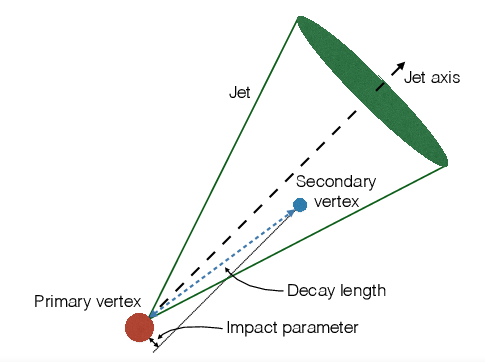
\includegraphics[width=0.5\textwidth]{figures/theoryFigs/b_tag_illustration.png}
 \centering
\caption{An illustration~\cite{Connelly2017PerformanceAC} of the production of a $b$-jet is shown. This illustrates the presence of a secondary vertex within a $b$-jet.}
\label{fig:btag-pic}
\end{figure}

In this analysis, we use the recommended DL1r (Deep-Learning Flavour Tagger) tagging algorithm~\cite{DL1r-slides}. The DL1r algorithm combines outputs from several low-level tagging algorithms using a Deep Neural Network and outputs the probability that a given input jet is identified as a $b$, $c$ or light flavoured jet.